\documentclass[UTF8,zihao=-4]{ctexart}

\usepackage[a4paper,margin=2.4cm]{geometry}
\usepackage{amsmath,amssymb,bm}
\usepackage{booktabs,longtable,tabularx,array,multirow}
\usepackage{graphicx}
\usepackage{xcolor}
\usepackage{float}
\usepackage{enumitem}
\usepackage{caption}
\usepackage{xurl}
\usepackage{hyperref}
\usepackage{titlesec}
\usepackage{fancyhdr}
\usepackage{siunitx}
\usepackage{makecell}

\graphicspath{{figures/}}

\definecolor{titleblue}{HTML}{0B2545}
\definecolor{headblue}{HTML}{1F4D78}
\definecolor{lightgray}{HTML}{F4F6F9}

\hypersetup{
  colorlinks=true,
  linkcolor=headblue,
  urlcolor=headblue,
  citecolor=headblue
}

\pagestyle{fancy}
\setlength{\headheight}{15pt}
\fancyhf{}
\lhead{基于 SNAP Facebook 社交网络的链路预测实验报告}
\rhead{\thepage}
\renewcommand{\headrulewidth}{0.4pt}

\titleformat{\section}{\Large\bfseries\color{headblue}}{\thesection}{0.6em}{}
\titleformat{\subsection}{\large\bfseries\color{headblue}}{\thesubsection}{0.6em}{}
\titleformat{\subsubsection}{\normalsize\bfseries\color{titleblue}}{\thesubsubsection}{0.6em}{}
\setlist[itemize]{leftmargin=2em,itemsep=0.2em,topsep=0.2em}
\setlist[enumerate]{leftmargin=2em,itemsep=0.2em,topsep=0.2em}
\renewcommand{\arraystretch}{1.25}
\emergencystretch=2em
\Urlmuskip=0mu plus 2mu
\captionsetup{font=small,labelfont=bf}
\newcolumntype{Y}{>{\raggedright\arraybackslash}X}
\newcolumntype{C}{>{\centering\arraybackslash}X}

\title{\bfseries\color{titleblue}基于 SNAP Facebook 社交网络的链路预测实验报告}
\author{徐元博 2025080901021 \&  叶信南 2025081001024}
\date{\today}

\begin{document}

\maketitle
\tableofcontents
\newpage

\begin{abstract}
本实验围绕社交网络中的好友关系预测任务展开。给定一个已经观测到的无向社交图
\(G=(V,E)\)，实验目标是根据已有边预测尚未观测到的潜在边，即判断两个当前未连接的用户未来或隐藏状态下是否可能存在好友关系。实验重点使用 SNAP Facebook Social Circles 数据集，并比较三类方法：基于人工结构指标的传统 baseline、图结构特征加 MLP、以及 LightGCN 表示学习模型。为补充说明模型在不同网络结构下的表现，实验还引入 ca-GrQc 论文合作网络和 email-Eu-core 邮件网络，并额外比较 Katz、MultiHop、DeepWalk、MF、GCN、GAT 等方法。

实验结果表明，在 Facebook 好友预测任务中，CN、AA、RA 等共同邻居类局部结构方法非常强，尤其 RA 在公平 Top-K 评测中取得最高 NDCG@10，达到 0.8947；MLP 的 NDCG@10 为 0.8886，接近 RA，但耗时明显更高；LightGCN 在多方法公平评测中的 Facebook NDCG@10 为 0.7437，低于传统启发式与 MLP。在独立的 LightGCN 五随机种子实验中，LightGCN 在 1:1 正负样本二分类评测下取得 Test AUC \(0.9923\pm0.0002\)、Test AP \(0.9909\pm0.0002\)。总体来看，在缺少有效节点属性、且任务本质是静态图隐藏边恢复时，简单但针对性强的局部结构方法仍然具有很高竞争力；LightGCN 的价值主要体现在端到端节点表示学习、可扩展到推荐系统场景，以及作为后续引入特征、时间信息和排序损失的基础模型。
\end{abstract}

\section{背景}

链路预测是网络科学和图机器学习中的经典问题。其核心任务是：已知图中一部分节点和边，预测哪些尚未连接的节点对最可能形成连接。在社交网络中，这一任务对应好友推荐；在论文合作网络中，对应潜在合作者预测；在邮件网络中，对应潜在通信关系预测。本实验任务为：给定已观测到的社交网络图，为当前不存在好友关系的用户对 \((u,v)\) 打分，分数越高表示两人越可能形成好友关系。

本实验选择 Facebook 社交网络作为重点数据集，原因是该网络具有明显的社交圈结构和三角闭包现象。所谓三角闭包，是指如果用户 A 和用户 B 具有很多共同好友，那么 A 与 B 成为好友的概率通常更高。因此，CN、AA、RA 等局部结构指标天然适合该任务。与此同时，图神经网络和推荐系统中的协同过滤方法也提供了另一种思路：不再手工设计共同邻居指标，而是直接学习每个节点的 embedding，再用向量相似度预测连边概率。LightGCN 正是这一路线的代表模型。

本实验的核心问题是：在 Facebook 好友预测任务中，人工图结构特征和 MLP 是否已经足够强？LightGCN 自动学习节点表示能否超过这些传统方法？

\section{模型原理}

\subsection{Baseline：传统结构指标}

传统 baseline 不进行参数训练，而是直接根据训练图 \(G_{\text{train}}\) 中的局部结构为候选边 \((u,v)\) 打分。所有指标都只在训练图上计算，不能使用验证集和测试集边，否则会产生信息泄漏。

设 \(N(u)\) 表示节点 \(u\) 在训练图中的邻居集合，\(d(u)=|N(u)|\)。本实验中的主要 baseline 包括表~\ref{tab:baseline-formulas}。

\begin{table}[H]
\centering
\caption{传统链路预测指标及其核心思想}
\label{tab:baseline-formulas}
\small
\begin{tabularx}{\textwidth}{>{\bfseries}p{1.8cm} C Y}
\toprule
指标 & 公式 & 核心思想 \\
\midrule
CN &
\[
CN(u,v)=|N(u)\cap N(v)|
\]
& 共同好友越多，越可能连接。\\
\addlinespace
Jaccard &
\[
Jaccard(u,v)=\frac{|N(u)\cap N(v)|}{|N(u)\cup N(v)|}
\]
& 共同好友占总邻居比例越高，关系越可能存在。\\
\addlinespace
AA &
\[
AA(u,v)=\sum_{z\in N(u)\cap N(v)}\frac{1}{\log d(z)}
\]
& 降低高度共同邻居的影响。\\
\addlinespace
RA &
\[
RA(u,v)=\sum_{z\in N(u)\cap N(v)}\frac{1}{d(z)}
\]
& 更强地惩罚高度共同邻居，强调稀缺共同好友。\\
\addlinespace
PA &
\[
PA(u,v)=d(u)\cdot d(v)
\]
& 高度节点之间更容易连接。\\
\addlinespace
HPI &
\[
HPI(u,v)=\frac{CN(u,v)}{\min(d(u),d(v))}
\]
& 共同邻居数除以较小度数。\\
\addlinespace
HDI &
\[
HDI(u,v)=\frac{CN(u,v)}{\max(d(u),d(v))}
\]
& 共同邻居数除以较大度数。\\
\bottomrule
\end{tabularx}
\end{table}

其中 CN、AA、RA 都属于共同邻居类方法。它们直接刻画好友推荐中最重要的局部机制：两个人如果共享较多好友，或共享的好友本身更稀缺，那么两人更可能存在连接。PA 是一个对照方法，它只利用节点流行度，不利用共同邻域结构，因此在本实验中表现较弱。

\subsection{图结构特征 + MLP}

MLP 方法不是直接从原始图中学习节点 embedding，而是先对候选边 \((u,v)\) 提取人工结构特征，再用多层感知机学习这些指标之间的非线性组合关系。根据 PPT 和实验方案，核心输入特征为
\[
x_{uv}=[CN,\ Jaccard,\ AA,\ RA,\ PA,\ HPI,\ HDI].
\]

在补充的多数据集公平评测代码中，MLP 特征进一步扩展为 9 维，包括 \(d(u)\)、\(d(v)\)、\(|d(u)-d(v)|\)、CN、Jaccard、AA、RA、PA 以及 HDI/HPI 的组合项。二者思想一致，都是将可解释的图结构指标输入 MLP。

MLP 的结构为
\[
\text{Input}\rightarrow 64\rightarrow 32\rightarrow 1.
\]
其中隐藏层使用 ReLU 激活和 dropout，输出层给出一个 logit：
\[
score(u,v)=MLP(x_{uv}).
\]
训练目标采用二元交叉熵损失：
\[
L=-y_{uv}\log\sigma(score(u,v))-(1-y_{uv})\log\left(1-\sigma(score(u,v))\right).
\]

\begin{figure}[H]
\centering
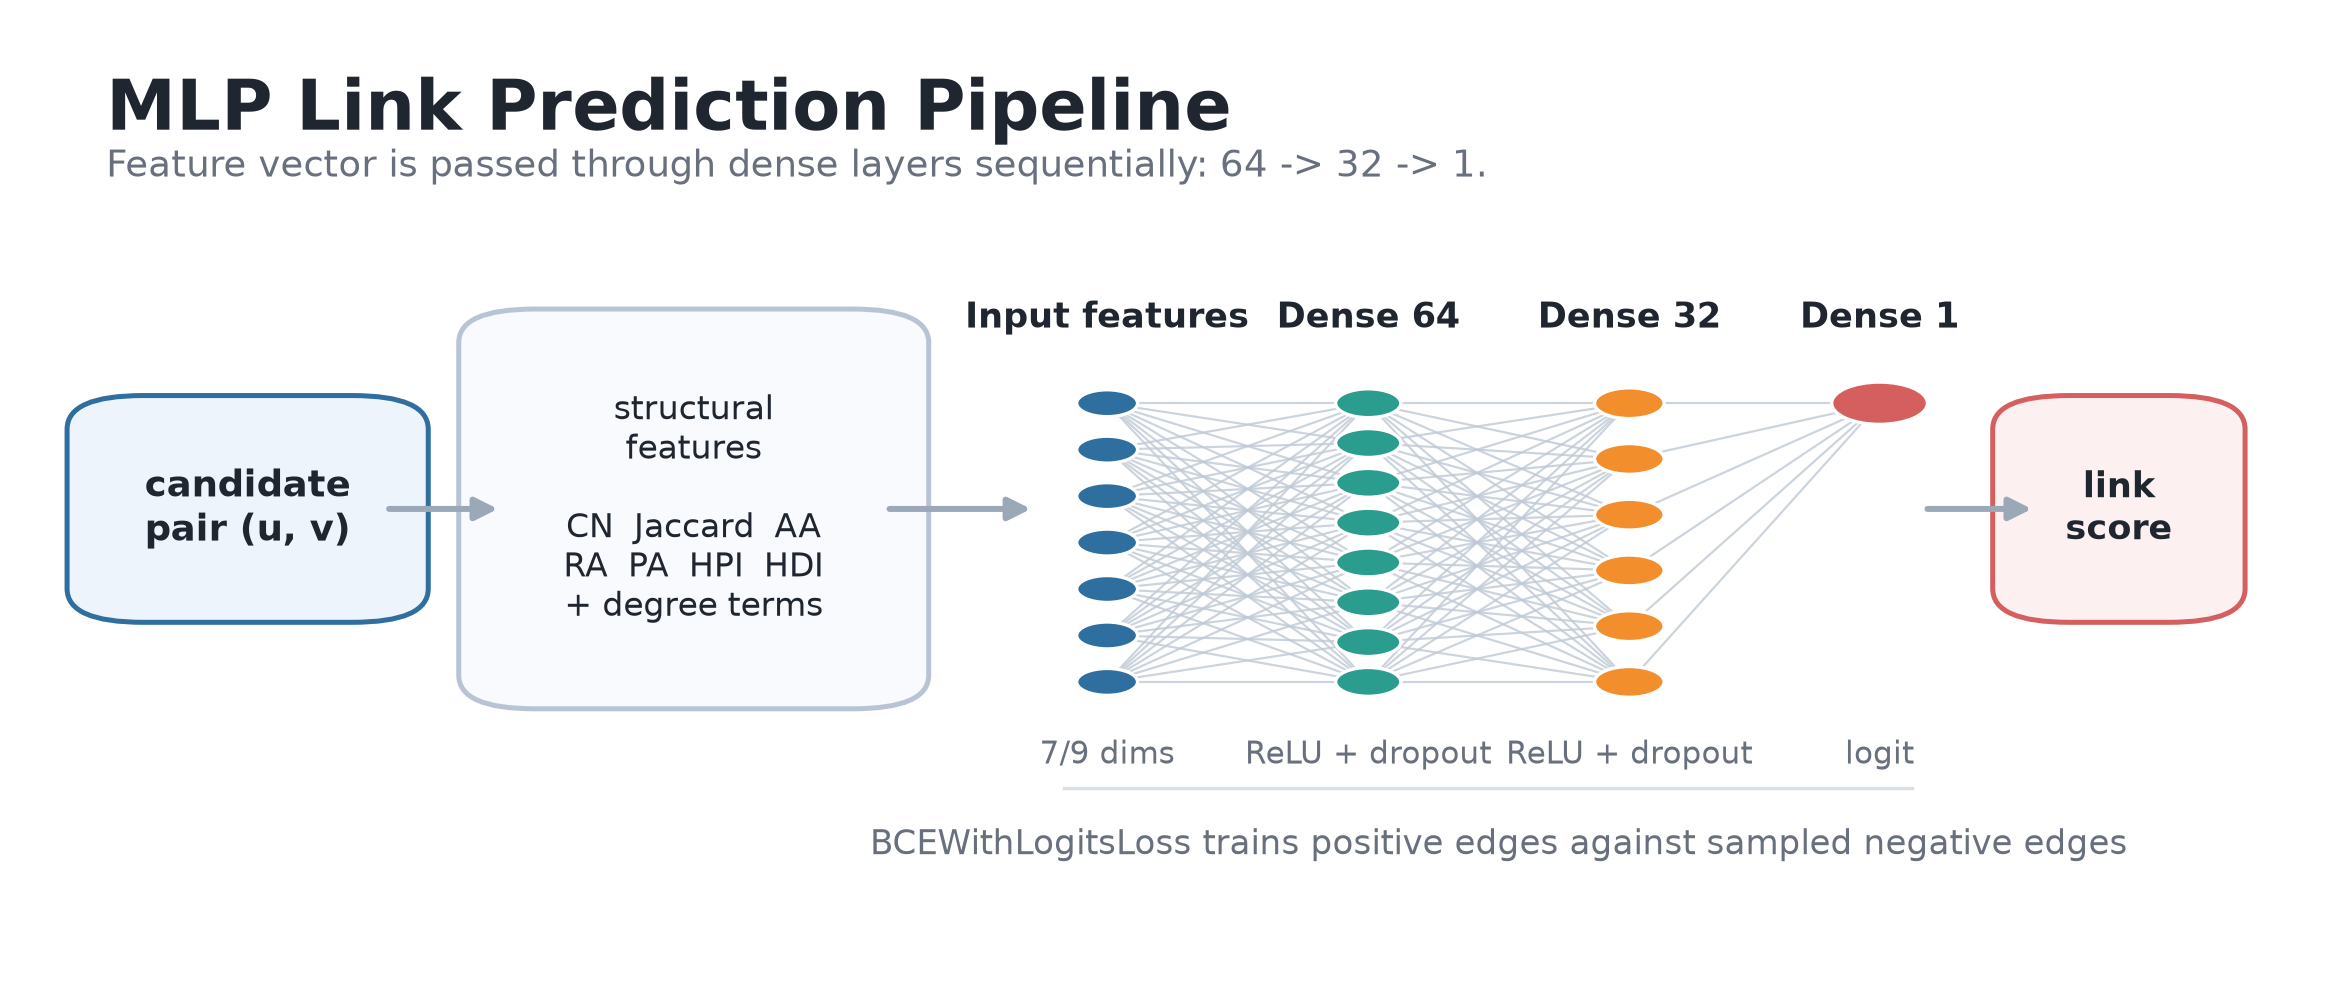
\includegraphics[width=0.92\textwidth]{mlp_schematic.png}
\caption{MLP 链路预测流程示意：先抽取候选边的结构特征，再经过两层隐藏层输出连边分数。}
\label{fig:mlp-schematic}
\end{figure}

MLP 的优势是输入特征可解释，同时能够学习多个结构指标之间的非线性组合。例如，RA 和 AA 已经对共同邻居进行了度数惩罚，而 MLP 可以学习在不同候选边上如何综合 CN、RA、Jaccard 和 PA 等信号。其不足是仍然依赖人工特征工程，且在较大候选集上需要先计算特征，时间成本高于直接打分的启发式方法。

\subsection{LightGCN}

LightGCN 是一种为推荐系统设计的轻量图卷积模型。与普通 GCN 不同，LightGCN 删除了特征变换和非线性激活，只保留邻居聚合这一核心操作。它的基本思想是：每个节点先拥有一个可训练的初始 embedding，然后在图上进行多层线性传播，最后将每一层 embedding 求平均作为节点最终表示。

在本实验中，Facebook 好友网络被看作无向同质图。节点初始向量为
\[
e_u^{(0)}\in\mathbb{R}^{d}.
\]
第 \(k\) 层传播为
\[
e_u^{(k+1)}
=
\sum_{v\in N(u)}
\frac{1}{\sqrt{d(u)d(v)}}e_v^{(k)}.
\]
最终节点表示为
\[
z_u=\frac{1}{K+1}\sum_{k=0}^{K}e_u^{(k)}.
\]
候选边打分采用点积：
\[
score(u,v)=z_u^\top z_v.
\]

\begin{figure}[H]
\centering
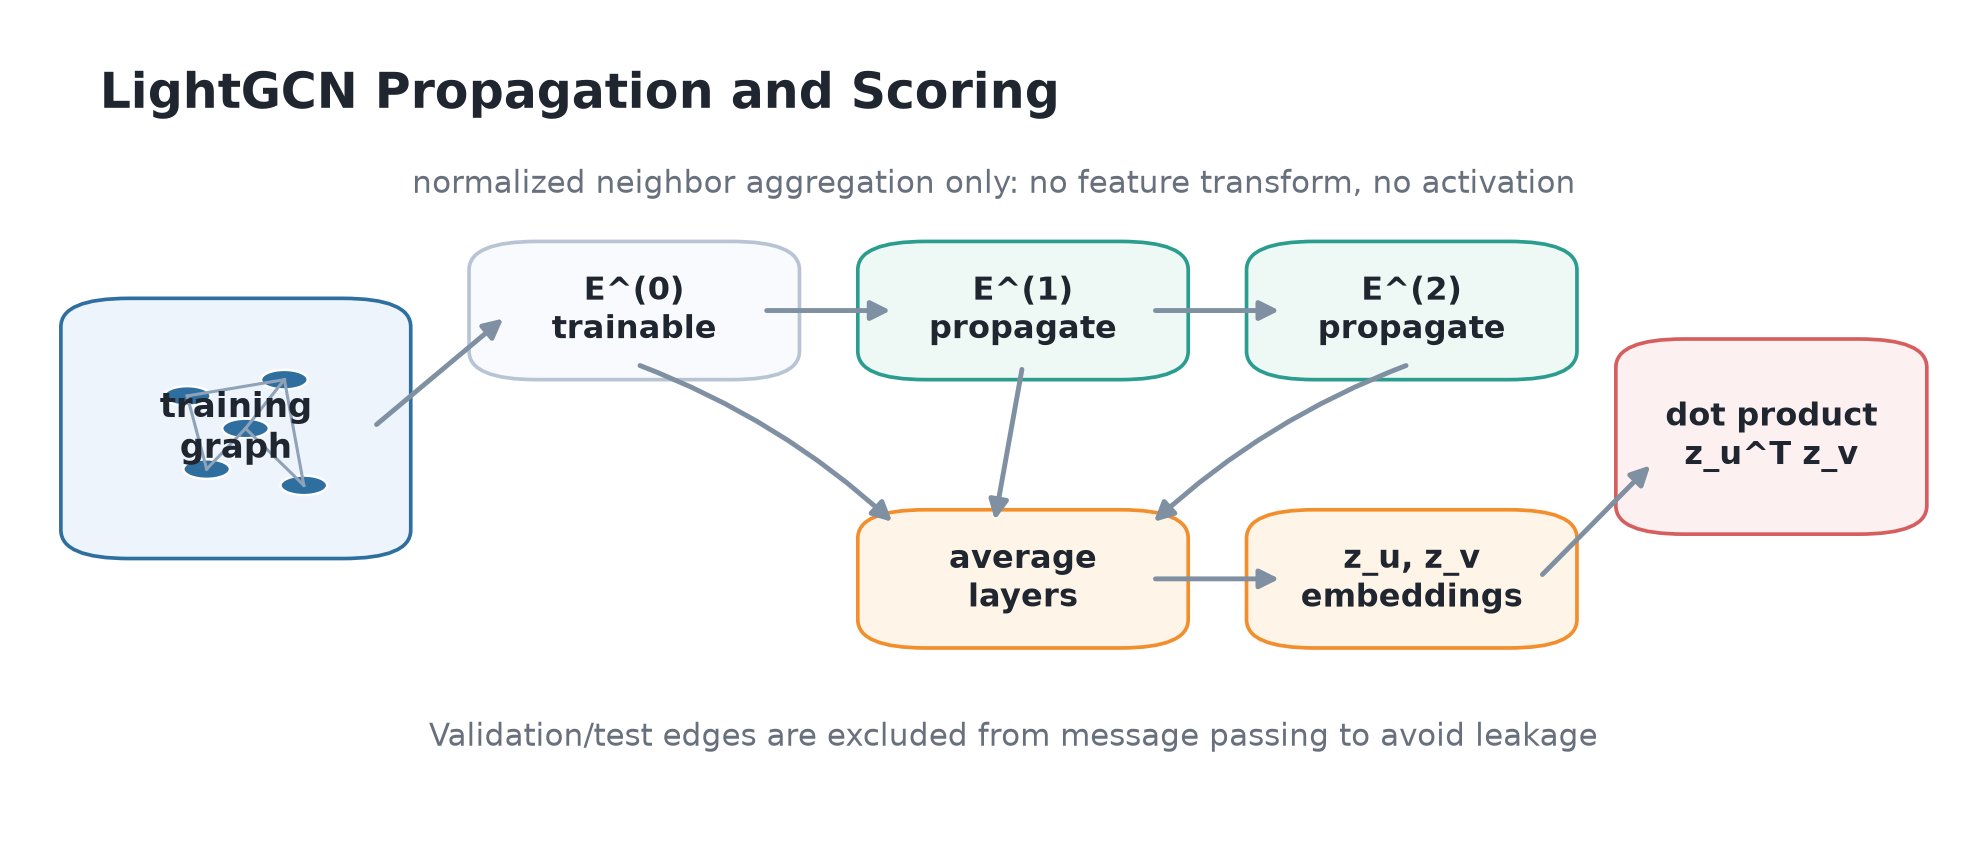
\includegraphics[width=0.92\textwidth]{lightgcn_schematic.png}
\caption{LightGCN 传播与打分示意：仅保留归一化邻居聚合，对各层 embedding 求平均后用点积预测候选边。}
\label{fig:lightgcn-schematic}
\end{figure}

代码实现中，\texttt{model.py} 的 \texttt{LightGCN} 类只包含一个节点 embedding 表，参数量约为 \(|V|\times d\)。对于 Facebook 数据集，节点数为 4039，embedding 维度为 64，因此参数量为
\[
4039\times64=258496.
\]
LightGCN 训练时同样使用正负样本二分类目标，损失函数为 \texttt{BCEWithLogitsLoss}。训练图只包含训练边，验证边和测试边不参与邻接矩阵传播，这是本实验中避免信息泄漏的关键设计。

\section{实验数据集}

\subsection{主数据集：SNAP Facebook Social Circles}

主实验使用 SNAP Facebook Social Circles 中的 \texttt{facebook\_combined.txt}。每一行表示一条无向好友边：
\begin{verbatim}
u v
\end{verbatim}
实验读取边列表后进行去重、去自环、节点重编号，并构造无向无权图。根据 SNAP 数据集页面和本地代码读取结果，该图包含表~\ref{tab:datasets-main} 所示规模。

\begin{table}[H]
\centering
\caption{主数据集信息}
\label{tab:datasets-main}
\begin{tabularx}{\textwidth}{lrrlY}
\toprule
数据集 & 节点数 & 边数 & 图类型 & 结构特点 \\
\midrule
Facebook & 4039 & 88234 & 无向社交网络 & 聚类系数高，三角闭包明显，适合好友预测。\\
\bottomrule
\end{tabularx}
\end{table}

SNAP 页面给出的 Facebook 平均聚类系数为 0.6055，三角形数量为 1,612,010，这说明网络局部团簇结构很强。因此，共同邻居类方法在该数据集上具有天然优势。

\subsection{补充数据集}

为说明结论不是只依赖 Facebook 单一网络，补充实验使用了两个 SNAP 数据集，见表~\ref{tab:datasets-extra}。

\begin{table}[H]
\centering
\caption{补充数据集信息}
\label{tab:datasets-extra}
\small
\begin{tabularx}{\textwidth}{lrrYY}
\toprule
数据集 & SNAP 原始节点数 & SNAP 原始边数 & 本实验处理 & 说明 \\
\midrule
ca-GrQc & 5242 & 14496 & 默认取最大连通分量 & arXiv GR-QC 论文合作网络。\\
email-Eu-core & 1005 & 25571 & 有向邮件网络转无向图，默认取最大连通分量 & 欧洲研究机构内部邮件通信网络。\\
\bottomrule
\end{tabularx}
\end{table}

ca-GrQc 的边表示两位作者是否共同发表论文。论文合作网络通常具有明显的小团体和 clique 结构，因此 CN 等共同邻居方法很强。email-Eu-core 的边表示机构成员之间至少有一次邮件通信，通信关系受到部门、职位和工作流影响，局部结构信号不如好友和合作网络纯粹，因此整体预测难度更高。

\section{实验过程}

\subsection{数据划分}

Facebook LightGCN 独立实验采用 80\% / 10\% / 10\% 的边划分比例，见表~\ref{tab:split}。

\begin{table}[H]
\centering
\caption{Facebook 数据划分}
\label{tab:split}
\begin{tabularx}{0.75\textwidth}{lrl}
\toprule
集合 & 数量 & 用途 \\
\midrule
训练边 & 70588 & 构建训练图并训练模型。\\
验证边 & 8823 & early stopping 和模型选择。\\
测试边 & 8823 & 最终评估。\\
\bottomrule
\end{tabularx}
\end{table}

代码中的 \texttt{split\_edges\_preserve\_connectivity} 会先通过并查集保留训练图的连通骨架，再划分剩余边。这样可以减少训练图中的孤立节点，使 LightGCN 在训练阶段能够为尽可能多的节点聚合邻居信息。

补充多数据集公平评测脚本采用 \texttt{val\_ratio=0.05}、\texttt{test\_ratio=0.10}，并默认只使用最大连通分量。该脚本用于比较 Facebook、ca-GrQc、email-Eu-core 上的 15 种方法，因此报告中将其作为跨方法、跨数据集的补充评测口径。

\subsection{负采样}

链路预测需要同时构造正样本和负样本。正样本来自真实边，负样本来自完整图中不存在边的节点对：
\[
(u,v)\notin E_{\text{full}}.
\]
这里必须使用完整图 \(E_{\text{full}}\) 判断负样本，而不能只使用训练图。因为验证边和测试边虽然不在训练图中，但它们仍然是真实边，如果将它们误采为负样本，就会污染训练或评估。

Facebook LightGCN 独立实验中，训练阶段每个 epoch 动态采样与训练正边数量相同的负边，即正负比例为 1:1；验证集和测试集也使用固定的 1:1 正负样本计算 AUC 和 AP。Top-K 推荐评估时，对每个用户排除自己和训练集中已有好友，再对候选节点打分排序。

多数据集公平评测中，Top-K 采用用户级候选采样：每条测试正边会转化为两个方向的用户推荐目标，并为每个用户采样若干非好友负候选。该设置更接近推荐排序评测，也能避免全量候选在多个模型上计算过慢。

\subsection{参数设置}

Facebook LightGCN 独立实验的主要参数如表~\ref{tab:params} 所示。

\begin{table}[H]
\centering
\caption{LightGCN 参数设置}
\label{tab:params}
\begin{tabularx}{0.7\textwidth}{lr}
\toprule
参数 & 取值 \\
\midrule
embedding dim & 64 \\
propagation layers & 2 \\
score function & dot product \\
optimizer & Adam \\
learning rate & 0.001 \\
weight decay & \(10^{-5}\) \\
batch size & 4096 \\
max epochs & 200 \\
early stopping patience & 20 \\
validation metric & AP \\
random seeds & 2024, 2025, 2026, 2027, 2028 \\
loss & BCEWithLogitsLoss \\
\bottomrule
\end{tabularx}
\end{table}

MLP 使用两层隐藏层，隐藏维度为 64 和 32，激活函数为 ReLU，dropout 为 0.2，输出一个 logit，同样使用 Adam 和二元交叉熵损失。传统 baseline 不需要训练，只需在训练图上计算结构指标并对候选边排序。

补充多数据集脚本中，神经模型统一采用 \texttt{dim=64}、\texttt{layers=2}、\texttt{epochs=200}、\texttt{patience=20}、weight decay=\(10^{-5}\)，默认学习率为 0.01，Top-K 评测使用 K=5 和 K=10。

\subsection{训练过程}

LightGCN 的训练流程由 \texttt{trainer.py} 控制：

\begin{enumerate}
  \item 固定随机种子，读取 Facebook 边列表。
  \item 去除自环和重复边，将节点重编号为 \(0,\dots,|V|-1\)。
  \item 按连通性保持策略划分训练、验证、测试正边。
  \item 使用完整图非边构造验证负样本和测试负样本。
  \item 基于训练边构造对称归一化邻接矩阵 \(\hat A\)。
  \item 初始化 LightGCN 节点 embedding。
  \item 每个 epoch 动态采样训练负边，与训练正边组成 1:1 训练集。
  \item 前向传播得到节点表示 \(z_u\)，用点积计算候选边分数。
  \item 使用 \texttt{BCEWithLogitsLoss} 反向传播，Adam 更新初始 embedding。
  \item 每轮在验证集上计算 AUC 和 AP，以 Val AP 保存最好模型。
  \item patience 轮无提升则 early stopping。
  \item 加载最好模型，在测试集计算 AUC、AP、Precision@K、Recall@K 和 NDCG@K。
\end{enumerate}

该流程中最重要的公平性控制是：训练图、人工特征和 LightGCN 的消息传播都只能使用训练边；验证边和测试边只在评估阶段出现。

\section{评价指标和实验结果}

\subsection{评价指标}

本实验使用两类指标。二分类指标用于评估模型能否把真实边排在随机负边前面：AUC 表示随机抽一条正边和一条负边时，正边分数更高的概率；AP 关注正样本在排序中的整体靠前程度。推荐排序指标用于评估 Top-K 好友推荐质量，包括 Precision@K、Recall@K、Hit@K、NDCG@K 和 MRR。其中 NDCG@10 和 Recall@10 更接近好友推荐场景，因此作为 Top-K 分析中的重点指标。

\subsection{Facebook 主结果：公平 Top-K 评测}

根据 \texttt{link\_prediction\_results\_summary.xlsx} 中 Facebook 结果，Top-K 评测的主要方法表现如表~\ref{tab:facebook-topk} 所示。

\begin{table}[H]
\centering
\caption{Facebook 公平 Top-K 评测结果}
\label{tab:facebook-topk}
\scriptsize
\begin{tabularx}{\textwidth}{lrrrrrrr}
\toprule
方法 & AUC & AP & P@10 & R@10 & Hit@10 & NDCG@10 & 时间/s \\
\midrule
RA & 0.9931 & 0.7686 & 0.4006 & 0.8835 & 0.9996 & 0.8947 & 2.11 \\
MLP & 0.9937 & 0.7875 & 0.4015 & 0.8814 & 0.9983 & 0.8886 & 79.17 \\
CN & 0.9886 & 0.6230 & 0.3937 & 0.8747 & 0.9997 & 0.8868 & 1.60 \\
AA & 0.9901 & 0.6554 & 0.3959 & 0.8778 & 0.9996 & 0.8863 & 2.09 \\
Katz & 0.9862 & 0.5953 & 0.3879 & 0.8618 & 0.9956 & 0.8588 & 0.61 \\
LightGCN & 0.9818 & 0.5770 & 0.3520 & 0.8039 & 0.9856 & 0.7437 & 11.05 \\
GAT & 0.9761 & 0.4802 & 0.3159 & 0.7290 & 0.9512 & 0.6211 & 28.76 \\
GCN & 0.9593 & 0.3949 & 0.2724 & 0.6071 & 0.8939 & 0.4949 & 44.29 \\
PA & 0.7076 & 0.0863 & 0.0471 & 0.0751 & 0.2249 & 0.0620 & 1.86 \\
\bottomrule
\end{tabularx}
\end{table}

图~\ref{fig:facebook-ndcg} 将 NDCG@10 结果可视化，突出 Facebook 主任务中 RA、MLP 与 LightGCN 的相对位置。

\begin{figure}[H]
\centering
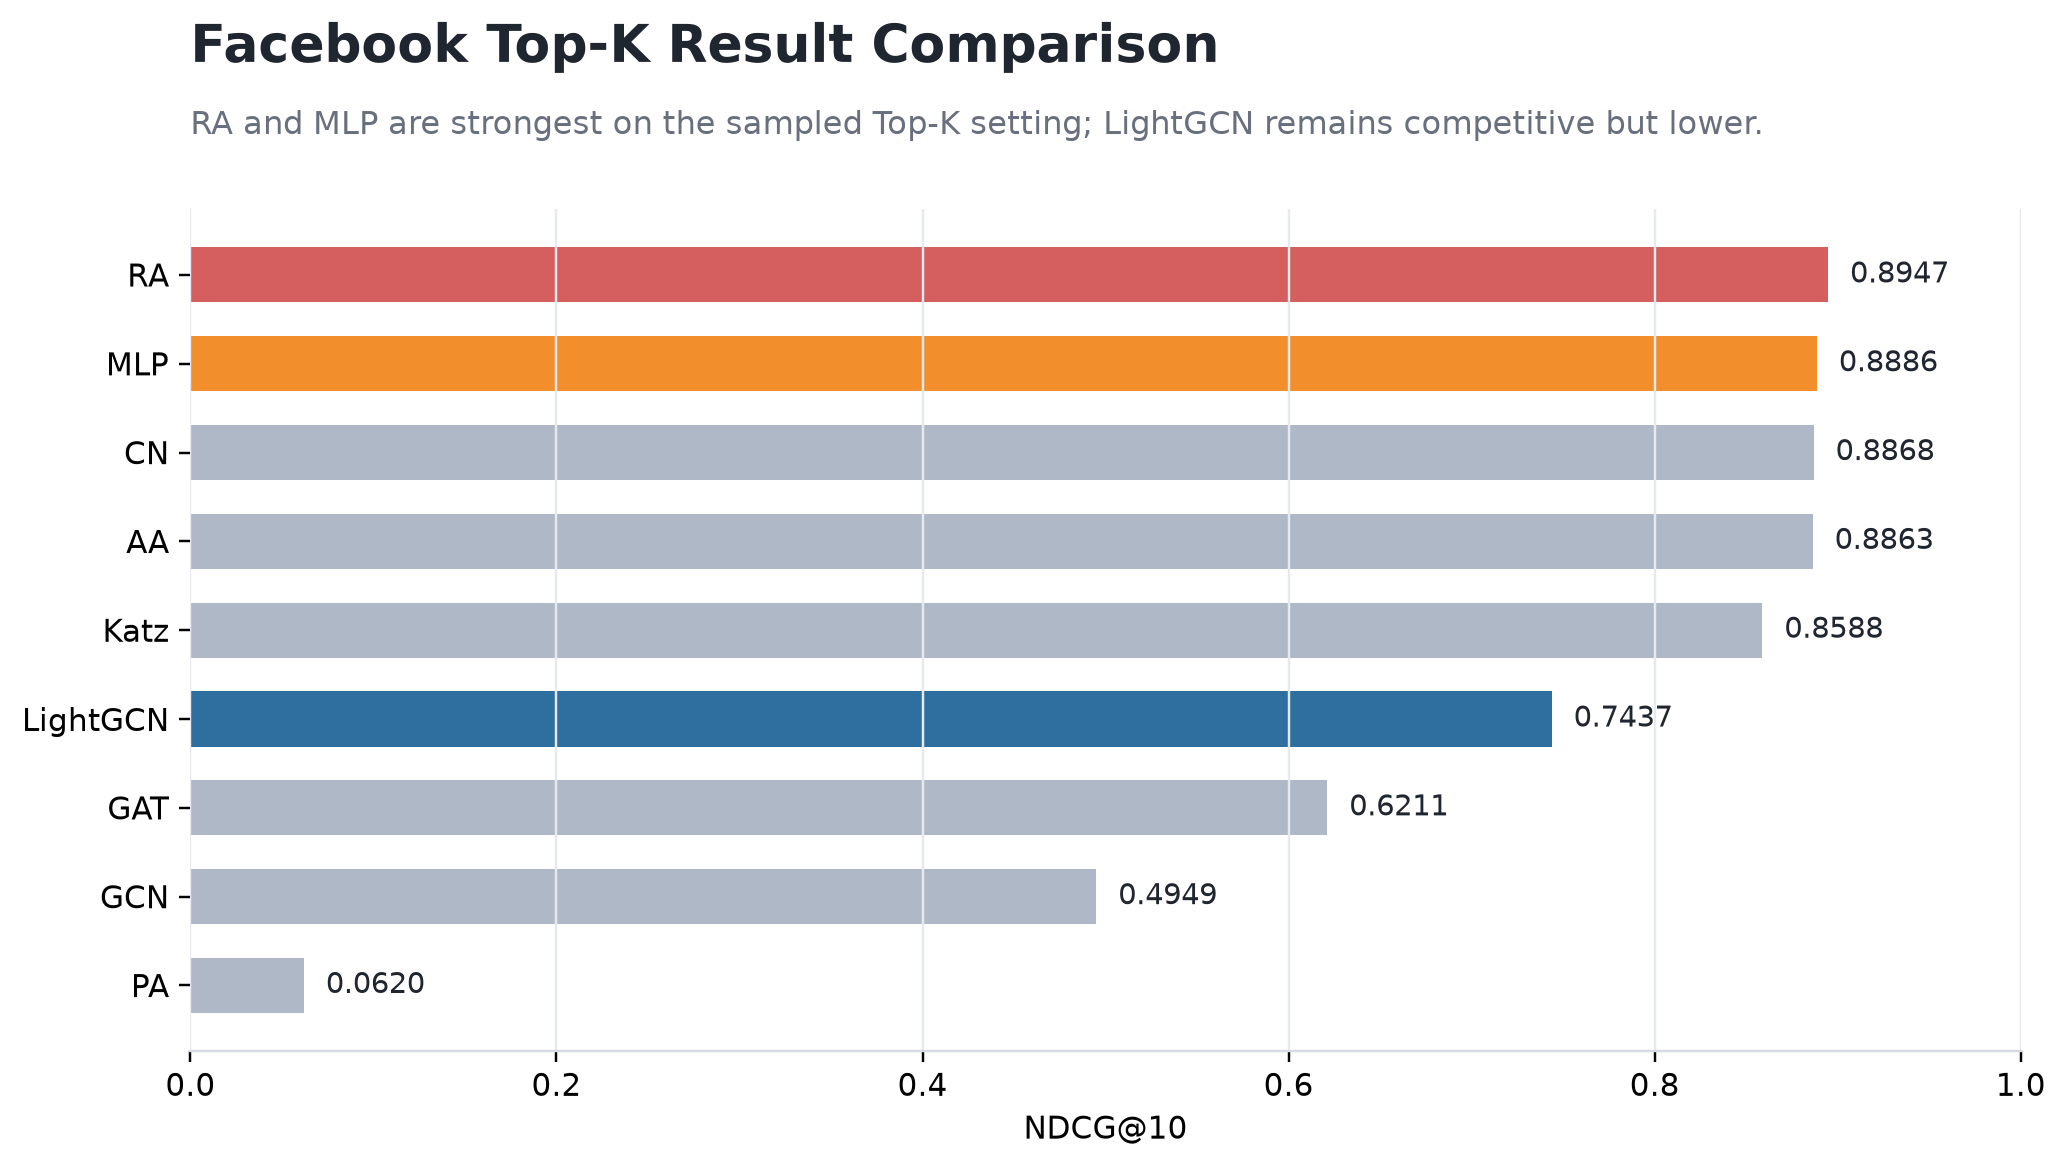
\includegraphics[width=0.94\textwidth]{facebook_ndcg_comparison.png}
\caption{Facebook 公平 Top-K 评测中不同方法的 NDCG@10 对比。RA 和 MLP 最接近最优，LightGCN 低于局部结构启发式但仍明显优于 GCN/GAT。}
\label{fig:facebook-ndcg}
\end{figure}

从结果看，RA 在 Facebook 上取得最优 NDCG@10，为 0.8947；MLP 非常接近，NDCG@10 为 0.8886，并且 AUC/AP 略高；CN 和 AA 也非常接近 RA。这说明 Facebook 好友预测高度依赖共同好友和三角闭包结构。LightGCN 能够学习到有效节点表示，但在这一静态无向好友图的 Top-K 评测中没有超过传统局部结构方法。

运行时间也值得注意。MLP 的 Facebook 平均耗时为 79.17 秒，约为 RA 的 37.6 倍；RA 只需 2.11 秒即可取得更高 NDCG@10。因此，如果只考虑 Facebook 静态好友预测，RA 的性价比最高。

\subsection{Facebook 二分类评测：baseline、MLP 与 LightGCN}

在 1:1 正负样本二分类口径下，\texttt{output\_mlp/metrics\_summary.csv} 给出 baseline 和 MLP 的五随机种子结果；LightGCN 独立输出给出对应的五随机种子结果。主要 AUC/AP 如表~\ref{tab:binary} 所示。

\begin{table}[H]
\centering
\caption{Facebook 二分类评测结果}
\label{tab:binary}
\begin{tabularx}{\textwidth}{lrrY}
\toprule
方法 & AUC & AP & 说明 \\
\midrule
MLP & \(0.9949\pm0.0005\) & \(0.9952\pm0.0004\) & 图结构特征融合效果最好。\\
RA & \(0.9945\pm0.0005\) & \(0.9942\pm0.0005\) & 最强传统启发式之一。\\
AA & \(0.9935\pm0.0005\) & \(0.9926\pm0.0005\) & 与 RA/CN 接近。\\
CN & \(0.9924\pm0.0005\) & \(0.9905\pm0.0005\) & 共同邻居数量已很强。\\
LightGCN & \(0.9923\pm0.0002\) & \(0.9909\pm0.0002\) & 独立 LightGCN 工程结果。\\
PA & \(0.8409\pm0.0038\) & \(0.8547\pm0.0029\) & 只看节点度，明显不足。\\
\bottomrule
\end{tabularx}
\end{table}

该口径下，MLP、RA、AA、CN、LightGCN 的 AUC/AP 都很高，说明随机负样本较容易与真实边区分。MLP 略优于 RA，说明在局部结构指标已经很强的基础上，MLP 能进一步学习特征组合。但从 Top-K 好友推荐角度看，RA 仍然更有优势，因为它排序效果更好且计算更快。

\subsection{LightGCN 专项结果}

你负责的 LightGCN 部分在 Facebook 上进行了 5 个随机种子实验。聚合结果如表~\ref{tab:lightgcn-special} 所示。

\begin{table}[H]
\centering
\caption{LightGCN 五随机种子专项结果}
\label{tab:lightgcn-special}
\begin{tabularx}{0.78\textwidth}{lr}
\toprule
指标 & mean \(\pm\) std \\
\midrule
Best epoch & \(164.8000\pm10.3537\) \\
Best Val AP & \(0.9905\pm0.0011\) \\
Test AUC & \(0.9923\pm0.0002\) \\
Test AP & \(0.9909\pm0.0002\) \\
Precision@10 & \(0.1326\pm0.0026\) \\
Recall@10 & \(0.2641\pm0.0039\) \\
NDCG@10 & \(0.2454\pm0.0036\) \\
Precision@20 & \(0.1054\pm0.0017\) \\
Recall@20 & \(0.3813\pm0.0064\) \\
NDCG@20 & \(0.2830\pm0.0040\) \\
\bottomrule
\end{tabularx}
\end{table}

LightGCN 在二分类指标上非常稳定，五个 seed 的 Test AUC 都在 0.9919 到 0.9925 之间，Test AP 都在 0.9905 到 0.9911 之间。这说明模型能够学习到有区分性的节点表示。但是在全量候选 Top-K 评估中，NDCG@10 只有约 0.2454。这一结果低于多数据集公平脚本中的采样候选 Top-K 数值，原因是两个评测候选集合不同：独立 LightGCN 工程对每个用户几乎在全图候选中排序，任务更难；多数据集脚本则为每个用户采样负候选，任务相对容易，也更便于多个模型公平比较。

因此，LightGCN 部分的合理结论是：模型在边二分类上表现稳定，但在真实好友推荐式的 Top-K 排序中还需要更适配的训练目标和候选生成策略。

\subsection{补充数据集结果}

在 ca-GrQc 和 email-Eu-core 上，Top-K 结果进一步验证了共同邻居类方法的稳定性，见表~\ref{tab:extra-results}。

\begin{table}[H]
\centering
\caption{补充数据集上的 Top-K 结果}
\label{tab:extra-results}
\small
\begin{tabularx}{\textwidth}{llrrrY}
\toprule
数据集 & 最优方法 & 最优 NDCG@10 & MLP NDCG@10 & LightGCN NDCG@10 \\
\midrule
ca-GrQc & CN & 0.9827 & 0.9168 & 0.8780 \\
email-Eu-core & RA & 0.6153 & 0.6123 & 0.4299 \\
\bottomrule
\end{tabularx}
\end{table}

\begin{figure}[H]
\centering
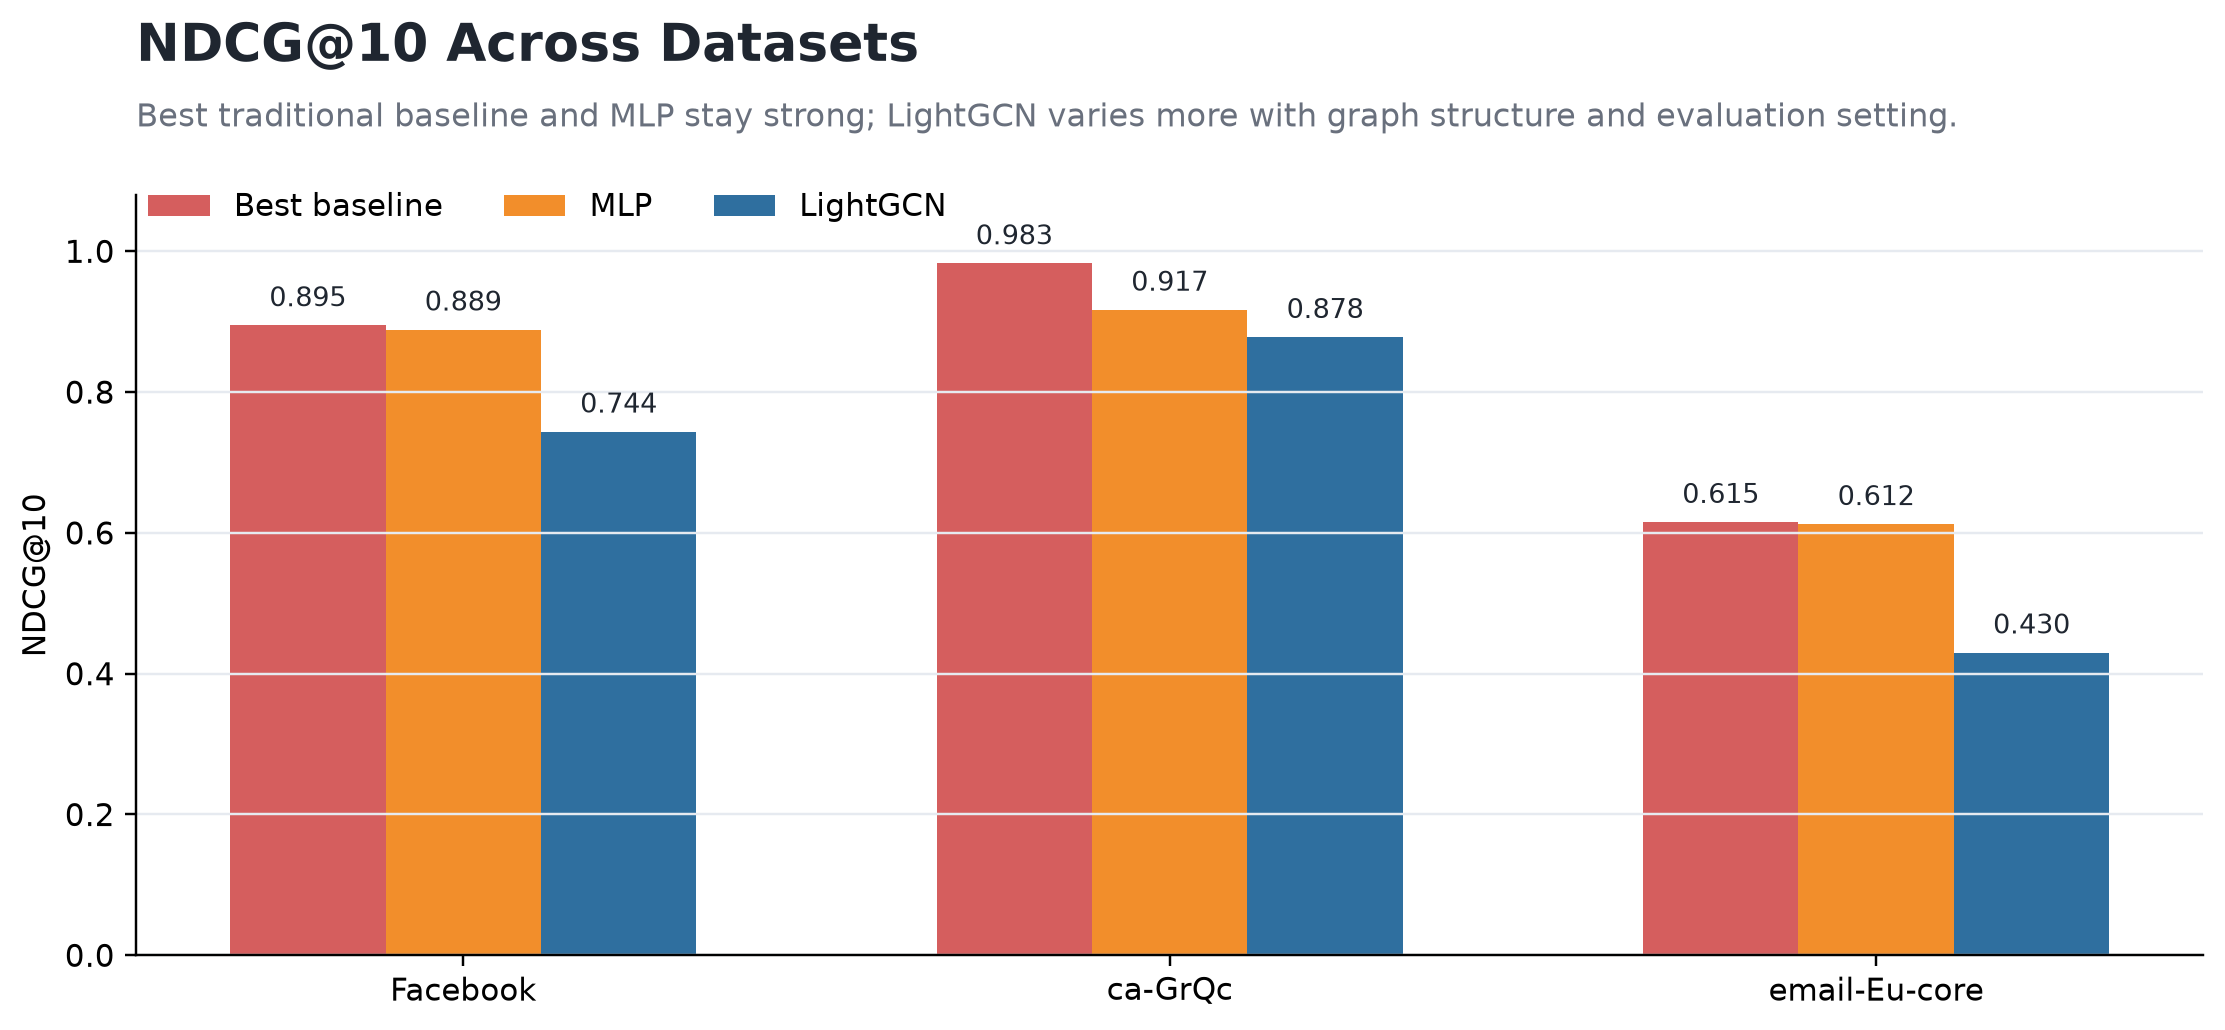
\includegraphics[width=0.94\textwidth]{cross_dataset_ndcg_summary.png}
\caption{三个数据集上最优传统 baseline、MLP 与 LightGCN 的 NDCG@10 对比。}
\label{fig:cross-dataset-ndcg}
\end{figure}

图~\ref{fig:cross-dataset-ndcg} 进一步展示了三类重点方法在不同网络结构下的趋势。共同邻居类 baseline 和 MLP 在三个数据集上都较稳，LightGCN 在 ca-GrQc 上表现较好，但在 email-Eu-core 上受网络机制差异影响更明显。

ca-GrQc 上 CN 最强，NDCG@10 达到 0.9827，说明论文合作网络中共同合作者数量本身就是非常强的信号。email-Eu-core 的最优 NDCG@10 只有 0.6153，明显低于 Facebook 和 ca-GrQc，说明邮件网络中的边不完全由局部社交圈决定，还可能受到部门、职位和工作流程影响。

综合三个数据集，平均 NDCG@10 排名前列的方法为 RA、CN、AA 和 MLP。RA 的平均 NDCG@10 为 0.8286，整体最稳；MLP 为 0.8059，表现强但耗时较高；LightGCN 平均 NDCG@10 为 0.6839，没有超过传统局部结构方法。

\section{分析和讨论}

\subsection{为什么传统局部结构方法很强}

Facebook 和 ca-GrQc 都具有明显的局部团簇结构。Facebook 中朋友之间往往共享社交圈，ca-GrQc 中论文合作者常形成研究小组或论文团队。对于这类网络，判断两点是否可能连边时，共同邻居数量和共同邻居质量非常关键。CN、AA、RA 正好直接编码了这一机制，因此不需要复杂训练也能取得很强结果。

RA 在 Facebook 和 email-Eu-core 上优于 CN，说明共同邻居数量之外，共同邻居的“稀缺性”也很重要。如果某个共同好友本身连接了很多人，那么它对判断两人是否属于同一小圈子的贡献应该降低；RA 用 \(1/d(w)\) 对共同邻居加权，恰好体现了这一点。

PA 的表现很差，说明“推荐高度节点”并不等价于好友预测。好友关系通常不是简单地连接热门用户，而是发生在局部社团内部。

\subsection{MLP 为什么接近最优}

MLP 将多个人工结构指标作为输入，相当于在强启发式特征上学习一个非线性组合器。它既保留了 CN、AA、RA 等指标的可解释性，又能够根据训练数据调整特征权重。因此在 Facebook 和 email-Eu-core 上，MLP 的结果非常接近 RA，甚至在 AUC/AP 上略高。

不过 MLP 的主要问题是计算成本。每个候选边都要先计算一组结构特征，当候选集合很大时，特征提取会成为瓶颈。从实验结果看，Facebook 上 MLP 耗时显著高于 RA，而排序效果并未超过 RA。因此，如果目标是快速构建强 baseline，RA 更合适；如果目标是学习多种结构信号的组合，MLP 更有价值。

\subsection{LightGCN 为什么没有超过 baseline}

LightGCN 的优势在推荐系统中通常体现在 user-item 二部图上，模型可以通过多层传播捕捉协同过滤信号。但本实验的 Facebook 是 user-user 同质图，并且没有使用可解释节点属性。此时模型只能从拓扑中学习 embedding，而 CN、AA、RA 已经非常直接地刻画了二跳邻域和三角闭包。

LightGCN 没有超过 baseline 的可能原因包括：
\begin{enumerate}
  \item 缺少节点特征。Facebook 数据集虽然原始版本包含匿名 profile features，但当前实验只使用 \texttt{facebook\_combined.txt} 边列表，没有使用节点属性。
  \item 训练目标和评估目标不完全一致。LightGCN 使用 BCE 做正负样本二分类，而最终关注的是每个用户的 Top-K 排序。二分类分数高不一定意味着全量候选排序最优。
  \item 随机负样本较容易。AUC/AP 使用 1:1 随机负边时，模型容易区分正边和负边；但 Top-K 推荐面对的是大量非好友候选，难度更高。
  \item 局部启发式命中任务机制。RA/CN/AA 直接计算共同邻居，而 LightGCN 的多层平均传播可能把局部精确信号平滑到 embedding 中，导致排序时不如显式指标。
  \item 模型场景存在差异。LightGCN 原本面向 user-item 推荐图，本实验将其用于 user-user 社交图，需要更细的负采样、loss 和层数调参。
\end{enumerate}

因此，本实验不能简单得出“GNN 不好”的结论。更准确的表述是：在缺少节点属性、以静态无向图隐藏边恢复为目标、且局部闭三角非常强的网络上，传统局部结构指标比当前设置下的 LightGCN 更有效。

\subsection{评测口径的局限}

本实验本质上是将静态图中的一部分边隐藏，再让模型恢复这些边。这与真实的未来好友预测并不完全相同。真实好友推荐更合理的评估方式应该按时间切分，例如用某一时刻之前的边训练，预测之后新出现的边。

此外，不同结果文件中存在两种 Top-K 口径：独立 LightGCN 工程使用更接近全量候选的评估，多数据集公平脚本使用采样候选评估。二者数值不能直接混为同一表格比较。因此报告中将独立 LightGCN 结果作为模型专项复现，将 \path{link_prediction_results_summary.xlsx} 作为跨方法公平比较。

\section{后续方向}

基于上述结果，后续工作不应只围绕“更换更复杂模型”展开，而应同时改进数据划分、训练目标、候选生成和模型输入，使实验口径更接近真实好友推荐场景。可优先从以下方向继续推进：

\begin{enumerate}
  \item 使用时间切分。若能获得带时间戳的边，应按时间顺序划分训练集和测试集，评估模型预测未来新增边的能力，而不是仅恢复静态图中被隐藏的边。这样得到的结论更接近真实好友推荐系统。
  \item 改进负采样。当前随机负采样相对容易，后续可以加入 hard negative sampling，例如采样二跳可达但不存在边的节点对，或按共同邻居数量分层采样负边，使训练任务更贴近 Top-K 推荐面对的大量相似候选。
  \item 使用排序损失。LightGCN 可进一步尝试 BPR loss、pairwise ranking loss 或 listwise loss，使训练目标从“判断边是否存在”转向“把真实边排到候选集前列”，从而更直接优化 Recall@K 和 NDCG@K。
  \item 引入节点属性。Facebook 原始数据包含匿名 profile features，email-Eu-core 包含部门标签。将节点属性与结构 embedding、共同邻居特征结合，有助于检验 GNN 和 MLP 是否能在单纯拓扑信息之外获得额外收益。
  \item 构建两阶段推荐框架。第一阶段使用 RA/CN 等低成本方法快速生成候选集，第二阶段使用 MLP 或 LightGCN 重新排序。该方案既保留传统指标的效率，又为学习模型提供更聚焦的候选空间。
  \item 做系统调参和消融。对 LightGCN 的 embedding 维度、传播层数、学习率、正则化强度、负采样策略以及是否加入 layer weights 进行系统实验；对 MLP 则可逐一移除 CN、AA、RA、PA 等特征，分析各结构信号的贡献。
  \item 保留有向和异质信息。email-Eu-core 原始图是有向邮件网络，转为无向图会损失发送和接收方向。后续可分别建模入边、出边，或使用有向图模型，以更好刻画通信网络中的角色差异。
  \item 进行显著性检验。对多 seed 结果进行统计检验，判断 RA、MLP 与 LightGCN 之间的差异是否显著，避免只凭均值差异作出过强结论。
\end{enumerate}

\section{总结}

本实验围绕链路预测中的好友推荐任务，完成了传统局部结构指标、图结构特征 MLP 与 LightGCN 的实现、复现和对比。结果表明，在 Facebook 这类具有强三角闭包和明显社交圈结构的网络中，共同邻居类方法仍然是非常强的基线。RA、CN、AA 能直接利用二跳邻域信息，在 Top-K 推荐中表现稳定，其中 RA 通过削弱高度数共同邻居的影响，进一步提升了排序质量。

MLP 的优势在于能够融合多种可解释结构特征，在 AUC/AP 等二分类指标上取得最优或接近最优结果，也说明人工结构指标之间确实存在可学习的非线性组合关系。但 MLP 需要为大量候选边计算特征，时间成本明显高于 RA 等简单启发式方法。因此，在小规模实验或追求更高精度时，MLP 具有价值；在需要快速生成候选集或构建强 baseline 时，RA 更加高效。

LightGCN 在 1:1 正负样本分类中取得稳定的高 AUC/AP，说明节点 embedding 能学习到有效的拓扑信息。不过，在更接近好友推荐的 Top-K 排序任务中，它没有超过 RA/CN/AA。造成这一现象的主要原因包括：当前实验缺少节点属性，LightGCN 的训练目标与排序评估目标不完全一致，随机负样本难度较低，以及传统局部指标已经高度契合本数据集中的闭三角机制。因此，本实验不能简单得出“图神经网络不适合链路预测”的结论，而应理解为：在静态、无属性、局部聚集性很强的社交图上，简单而可解释的局部结构方法可能比当前配置下的表示学习模型更有效。

补充的 ca-GrQc 和 email-Eu-core 实验进一步扩展了这一结论。合作网络中的共同邻居信号同样很强，而邮件网络受到组织结构、工作流程和方向性关系影响，预测难度明显更高。综合来看，本实验的核心结论是：传统共同邻居类方法是最稳健的基线，MLP 能在结构特征融合上进一步逼近最优结果，LightGCN 则具有继续扩展的潜力，但需要更合适的负采样、排序损失、节点属性和候选生成策略，才能在真实 Top-K 推荐场景中充分发挥优势。

\section{参考文献}

\begin{enumerate}[label={[\arabic*]}]
  \item SNAP. Social circles: Facebook dataset. \url{https://snap.stanford.edu/data/ego-Facebook.html}
  \item Julian McAuley and Jure Leskovec. Learning to Discover Social Circles in Ego Networks. NIPS, 2012. \url{https://arxiv.org/abs/1210.8182}
  \item SNAP. General Relativity and Quantum Cosmology collaboration network. \url{https://snap.stanford.edu/data/ca-GrQc.html}
  \item SNAP. email-Eu-core network. \url{https://snap.stanford.edu/data/email-Eu-core.html}
  \item David Liben-Nowell and Jon Kleinberg. The Link-Prediction Problem for Social Networks. Journal of the American Society for Information Science and Technology, 2007. \url{https://doi.org/10.1002/asi.20591}
  \item Lada A. Adamic and Eytan Adar. Friends and Neighbors on the Web. Social Networks, 2003. \url{https://doi.org/10.1016/S0378-8733(03)00009-1}
  \item Tao Zhou, Linyuan Lu, and Yi-Cheng Zhang. Predicting Missing Links via Local Information. European Physical Journal B, 2009. \url{https://arxiv.org/abs/0901.0553}
  \item Xiangnan He, Kuan Deng, Xiang Wang, Yan Li, Yongdong Zhang, and Meng Wang. LightGCN: Simplifying and Powering Graph Convolution Network for Recommendation. SIGIR, 2020. \url{https://arxiv.org/abs/2002.02126}
  \item Thomas N. Kipf and Max Welling. Semi-Supervised Classification with Graph Convolutional Networks. ICLR, 2017. \url{https://arxiv.org/abs/1609.02907}
  \item Petar Velickovic, Guillem Cucurull, Arantxa Casanova, Adriana Romero, Pietro Lio, and Yoshua Bengio. Graph Attention Networks. ICLR, 2018. \url{https://arxiv.org/abs/1710.10903}
\end{enumerate}

\section{代码}
shawnxyb. Link Prediction Projects: experiment code repository. GitHub. \url{https://github.com/shawnxyb/link-prediction-projects}

\end{document}
